% Options for packages loaded elsewhere
% Options for packages loaded elsewhere
\PassOptionsToPackage{unicode}{hyperref}
\PassOptionsToPackage{hyphens}{url}
\PassOptionsToPackage{dvipsnames,svgnames,x11names}{xcolor}
%
\documentclass[
  letterpaper,
  DIV=11,
  numbers=noendperiod]{scrartcl}
\usepackage{xcolor}
\usepackage{amsmath,amssymb}
\setcounter{secnumdepth}{5}
\usepackage{iftex}
\ifPDFTeX
  \usepackage[T1]{fontenc}
  \usepackage[utf8]{inputenc}
  \usepackage{textcomp} % provide euro and other symbols
\else % if luatex or xetex
  \usepackage{unicode-math} % this also loads fontspec
  \defaultfontfeatures{Scale=MatchLowercase}
  \defaultfontfeatures[\rmfamily]{Ligatures=TeX,Scale=1}
\fi
\usepackage{lmodern}
\ifPDFTeX\else
  % xetex/luatex font selection
\fi
% Use upquote if available, for straight quotes in verbatim environments
\IfFileExists{upquote.sty}{\usepackage{upquote}}{}
\IfFileExists{microtype.sty}{% use microtype if available
  \usepackage[]{microtype}
  \UseMicrotypeSet[protrusion]{basicmath} % disable protrusion for tt fonts
}{}
\makeatletter
\@ifundefined{KOMAClassName}{% if non-KOMA class
  \IfFileExists{parskip.sty}{%
    \usepackage{parskip}
  }{% else
    \setlength{\parindent}{0pt}
    \setlength{\parskip}{6pt plus 2pt minus 1pt}}
}{% if KOMA class
  \KOMAoptions{parskip=half}}
\makeatother
% Make \paragraph and \subparagraph free-standing
\makeatletter
\ifx\paragraph\undefined\else
  \let\oldparagraph\paragraph
  \renewcommand{\paragraph}{
    \@ifstar
      \xxxParagraphStar
      \xxxParagraphNoStar
  }
  \newcommand{\xxxParagraphStar}[1]{\oldparagraph*{#1}\mbox{}}
  \newcommand{\xxxParagraphNoStar}[1]{\oldparagraph{#1}\mbox{}}
\fi
\ifx\subparagraph\undefined\else
  \let\oldsubparagraph\subparagraph
  \renewcommand{\subparagraph}{
    \@ifstar
      \xxxSubParagraphStar
      \xxxSubParagraphNoStar
  }
  \newcommand{\xxxSubParagraphStar}[1]{\oldsubparagraph*{#1}\mbox{}}
  \newcommand{\xxxSubParagraphNoStar}[1]{\oldsubparagraph{#1}\mbox{}}
\fi
\makeatother

\usepackage{color}
\usepackage{fancyvrb}
\newcommand{\VerbBar}{|}
\newcommand{\VERB}{\Verb[commandchars=\\\{\}]}
\DefineVerbatimEnvironment{Highlighting}{Verbatim}{commandchars=\\\{\}}
% Add ',fontsize=\small' for more characters per line
\usepackage{framed}
\definecolor{shadecolor}{RGB}{241,243,245}
\newenvironment{Shaded}{\begin{snugshade}}{\end{snugshade}}
\newcommand{\AlertTok}[1]{\textcolor[rgb]{0.68,0.00,0.00}{#1}}
\newcommand{\AnnotationTok}[1]{\textcolor[rgb]{0.37,0.37,0.37}{#1}}
\newcommand{\AttributeTok}[1]{\textcolor[rgb]{0.40,0.45,0.13}{#1}}
\newcommand{\BaseNTok}[1]{\textcolor[rgb]{0.68,0.00,0.00}{#1}}
\newcommand{\BuiltInTok}[1]{\textcolor[rgb]{0.00,0.23,0.31}{#1}}
\newcommand{\CharTok}[1]{\textcolor[rgb]{0.13,0.47,0.30}{#1}}
\newcommand{\CommentTok}[1]{\textcolor[rgb]{0.37,0.37,0.37}{#1}}
\newcommand{\CommentVarTok}[1]{\textcolor[rgb]{0.37,0.37,0.37}{\textit{#1}}}
\newcommand{\ConstantTok}[1]{\textcolor[rgb]{0.56,0.35,0.01}{#1}}
\newcommand{\ControlFlowTok}[1]{\textcolor[rgb]{0.00,0.23,0.31}{\textbf{#1}}}
\newcommand{\DataTypeTok}[1]{\textcolor[rgb]{0.68,0.00,0.00}{#1}}
\newcommand{\DecValTok}[1]{\textcolor[rgb]{0.68,0.00,0.00}{#1}}
\newcommand{\DocumentationTok}[1]{\textcolor[rgb]{0.37,0.37,0.37}{\textit{#1}}}
\newcommand{\ErrorTok}[1]{\textcolor[rgb]{0.68,0.00,0.00}{#1}}
\newcommand{\ExtensionTok}[1]{\textcolor[rgb]{0.00,0.23,0.31}{#1}}
\newcommand{\FloatTok}[1]{\textcolor[rgb]{0.68,0.00,0.00}{#1}}
\newcommand{\FunctionTok}[1]{\textcolor[rgb]{0.28,0.35,0.67}{#1}}
\newcommand{\ImportTok}[1]{\textcolor[rgb]{0.00,0.46,0.62}{#1}}
\newcommand{\InformationTok}[1]{\textcolor[rgb]{0.37,0.37,0.37}{#1}}
\newcommand{\KeywordTok}[1]{\textcolor[rgb]{0.00,0.23,0.31}{\textbf{#1}}}
\newcommand{\NormalTok}[1]{\textcolor[rgb]{0.00,0.23,0.31}{#1}}
\newcommand{\OperatorTok}[1]{\textcolor[rgb]{0.37,0.37,0.37}{#1}}
\newcommand{\OtherTok}[1]{\textcolor[rgb]{0.00,0.23,0.31}{#1}}
\newcommand{\PreprocessorTok}[1]{\textcolor[rgb]{0.68,0.00,0.00}{#1}}
\newcommand{\RegionMarkerTok}[1]{\textcolor[rgb]{0.00,0.23,0.31}{#1}}
\newcommand{\SpecialCharTok}[1]{\textcolor[rgb]{0.37,0.37,0.37}{#1}}
\newcommand{\SpecialStringTok}[1]{\textcolor[rgb]{0.13,0.47,0.30}{#1}}
\newcommand{\StringTok}[1]{\textcolor[rgb]{0.13,0.47,0.30}{#1}}
\newcommand{\VariableTok}[1]{\textcolor[rgb]{0.07,0.07,0.07}{#1}}
\newcommand{\VerbatimStringTok}[1]{\textcolor[rgb]{0.13,0.47,0.30}{#1}}
\newcommand{\WarningTok}[1]{\textcolor[rgb]{0.37,0.37,0.37}{\textit{#1}}}

\usepackage{longtable,booktabs,array}
\usepackage{calc} % for calculating minipage widths
% Correct order of tables after \paragraph or \subparagraph
\usepackage{etoolbox}
\makeatletter
\patchcmd\longtable{\par}{\if@noskipsec\mbox{}\fi\par}{}{}
\makeatother
% Allow footnotes in longtable head/foot
\IfFileExists{footnotehyper.sty}{\usepackage{footnotehyper}}{\usepackage{footnote}}
\makesavenoteenv{longtable}
\usepackage{graphicx}
\makeatletter
\newsavebox\pandoc@box
\newcommand*\pandocbounded[1]{% scales image to fit in text height/width
  \sbox\pandoc@box{#1}%
  \Gscale@div\@tempa{\textheight}{\dimexpr\ht\pandoc@box+\dp\pandoc@box\relax}%
  \Gscale@div\@tempb{\linewidth}{\wd\pandoc@box}%
  \ifdim\@tempb\p@<\@tempa\p@\let\@tempa\@tempb\fi% select the smaller of both
  \ifdim\@tempa\p@<\p@\scalebox{\@tempa}{\usebox\pandoc@box}%
  \else\usebox{\pandoc@box}%
  \fi%
}
% Set default figure placement to htbp
\def\fps@figure{htbp}
\makeatother





\setlength{\emergencystretch}{3em} % prevent overfull lines

\providecommand{\tightlist}{%
  \setlength{\itemsep}{0pt}\setlength{\parskip}{0pt}}



 


% Colors and section styling
\usepackage{sectsty}
\usepackage{xcolor}
\definecolor{sectionblue}{HTML}{2563eb}
\sectionfont{\color{sectionblue}\bfseries\Large}
\subsectionfont{\color{sectionblue}\bfseries\large}

% Title styling
\usepackage{titling}
\pretitle{\begin{center}\Huge\bfseries\color{sectionblue}}
\posttitle{\par\end{center}\vskip 0.5em}
\preauthor{\begin{center}\large}
\postauthor{\par\end{center}}
\predate{\begin{center}\small}
\postdate{\par\end{center}}

% Code block styling via Shaded redefinition
\usepackage{tcolorbox}
\definecolor{codebg}{HTML}{F0F8FF}
\renewenvironment{Shaded}{%
  \begin{tcolorbox}[%
    colback=codebg,%
    colframe=codebg,%
    borderline west={3pt}{0pt}{sectionblue},%
    boxrule=0pt,%
    arc=0pt,%
    boxsep=5pt,%
    left=2mm,%
    right=2mm,%
    top=2mm,%
    bottom=2mm% 
  ]% 
}{%
  \end{tcolorbox}%
}
\KOMAoption{captions}{tableheading}
\makeatletter
\@ifpackageloaded{caption}{}{\usepackage{caption}}
\AtBeginDocument{%
\ifdefined\contentsname
  \renewcommand*\contentsname{Table of contents}
\else
  \newcommand\contentsname{Table of contents}
\fi
\ifdefined\listfigurename
  \renewcommand*\listfigurename{List of Figures}
\else
  \newcommand\listfigurename{List of Figures}
\fi
\ifdefined\listtablename
  \renewcommand*\listtablename{List of Tables}
\else
  \newcommand\listtablename{List of Tables}
\fi
\ifdefined\figurename
  \renewcommand*\figurename{Figure}
\else
  \newcommand\figurename{Figure}
\fi
\ifdefined\tablename
  \renewcommand*\tablename{Table}
\else
  \newcommand\tablename{Table}
\fi
}
\@ifpackageloaded{float}{}{\usepackage{float}}
\floatstyle{ruled}
\@ifundefined{c@chapter}{\newfloat{codelisting}{h}{lop}}{\newfloat{codelisting}{h}{lop}[chapter]}
\floatname{codelisting}{Listing}
\newcommand*\listoflistings{\listof{codelisting}{List of Listings}}
\makeatother
\makeatletter
\makeatother
\makeatletter
\@ifpackageloaded{caption}{}{\usepackage{caption}}
\@ifpackageloaded{subcaption}{}{\usepackage{subcaption}}
\makeatother
\makeatletter
\definecolor{QuartoInternalColor1}{rgb}{0.91,0.36,0.35}
\makeatother
\usepackage{bookmark}
\IfFileExists{xurl.sty}{\usepackage{xurl}}{} % add URL line breaks if available
\urlstyle{same}
\hypersetup{
  pdftitle={AI Pipeline Report},
  colorlinks=true,
  linkcolor={blue},
  filecolor={Maroon},
  citecolor={Blue},
  urlcolor={Blue},
  pdfcreator={LaTeX via pandoc}}


\title{AI Pipeline Report}
\author{}
\date{}
\begin{document}
\maketitle

\renewcommand*\contentsname{Table of contents}
{
\hypersetup{linkcolor=}
\setcounter{tocdepth}{3}
\tableofcontents
}

\begin{Shaded}
\begin{Highlighting}[]
\ImportTok{import}\NormalTok{ sys}
\ImportTok{from}\NormalTok{ pathlib }\ImportTok{import}\NormalTok{ Path}

\CommentTok{\# Add the src directory to Python path for importing project modules}
\NormalTok{sys.path.append(}\BuiltInTok{str}\NormalTok{(Path.cwd().parent }\OperatorTok{/} \StringTok{\textquotesingle{}src\textquotesingle{}}\NormalTok{))}
\end{Highlighting}
\end{Shaded}

Project Template: End-to-End AI/ML Pipeline

A reusable notebook scaffold for DS projects --- ingestion,
preprocessing, EDA, modeling, training, evaluation.

Table of Contents

\begin{itemize}
\tightlist
\item
  Project Introduction
\item
  Data Loading \& Initial Inspection
\item
  Preprocess
\item
  Exploratory Data Analysis
\item
  Feature Engineering
\item
  Models
\item
  Training
\item
  Evaluation
\item
  Conclusions \& Next Steps
\item
  Resources
\end{itemize}

Project Introduction

\begin{itemize}
\tightlist
\item
  Objectives \& Success Criteria: Define the problem, audience,
  constraints, and what ``good'' looks like.
\item
  Metrics vs business KPIs; target thresholds; baseline to beat.
\item
  Assumptions \& Scope: What's in/out, data coverage period,
  granularity, known limitations.
\end{itemize}

\begin{center}\rule{0.5\linewidth}{0.5pt}\end{center}

\begin{itemize}
\tightlist
\item
  Goal: Describe the problem you are solving, who benefits, and how
  success is measured.
\item
  Scope: Outline the boundaries (what is in/out) and key assumptions.
\item
  KPIs \& Metrics: Define primary metrics (e.g., accuracy, F1, AUC,
  MAPE) and business KPIs.
\item
  Risks \& Constraints: Data availability/quality, latency/cost
  constraints, privacy/compliance.
\end{itemize}

For example: - \textbf{Goal.} Train a \textbf{compact CycleGAN} that
translates \textbf{photos → Monet style}, then generate a Kaggle‑ready
submission (\texttt{images.zip}, 7,000--10,000 images @ 256×256).

\begin{itemize}
\tightlist
\item
  \textbf{Deliverables}

  \begin{itemize}
  \tightlist
  \item
    \textbf{Notebook (this file):} EDA → pipeline → model → training →
    generation → zip → discussion.
  \item
    \textbf{GitHub repo:} add this notebook + README + helper scripts.
  \item
    \textbf{Kaggle leaderboard screenshot:} after submitting
    \texttt{images.zip}.
  \end{itemize}
\item
  \textbf{Why CycleGAN?} Unpaired image‑to‑image translation fits this
  task: we have Monet paintings and photos but no aligned pairs. We keep
  the implementation compact and trainable on a modest GPU.
\end{itemize}

Data Loading \& Initial Inspection

Data Card (short): Sources, ownership, update cadence, schema summary,
PII/sensitive fields, licensing.

\begin{center}\rule{0.5\linewidth}{0.5pt}\end{center}

Load data, take a sneek preview Tell about the data, for instance:

To kick off our analysis, we'll load both the BBC News training set
(with labels) and the test set (without labels), then merge them into
one DataFrame. By combining all articles before any preprocessing, we
guarantee that every document --- whether destined for model fitting or
held out for final scoring --- passes through the exact same cleaning
and feature-extraction pipeline. Because our core modeling (TF--IDF
vectorization + NMF topic extraction) is entirely unsupervised, it never
``looks at'' the test labels, so there's no risk of leaking label
information. Instead, including test articles up front: • Ensures
Consistency: Every token is lowercased, stemmed, and filtered for
stop-words in the same way, avoiding any inadvertent vocabulary gaps
between train and test. • Boosts Coverage: Rare words that appear only
in test articles still become part of our TF--IDF vocabulary and topic
bases, making our latent factors richer and more robust.

After cleaning and factorization, we'll split back into train/test for
hyperparameter tuning (using only train labels) and a final, held-out
evaluation on the test labels.

\begin{Shaded}
\begin{Highlighting}[]
\ImportTok{import}\NormalTok{ sys}
\ImportTok{from}\NormalTok{ pathlib }\ImportTok{import}\NormalTok{ Path}
\NormalTok{sys.path.append(}\BuiltInTok{str}\NormalTok{(Path.cwd() }\OperatorTok{/} \StringTok{"src"}\NormalTok{))}

\ImportTok{import}\NormalTok{ pandas }\ImportTok{as}\NormalTok{ pd}
\ImportTok{import}\NormalTok{ matplotlib.pyplot }\ImportTok{as}\NormalTok{ plt}
\ImportTok{from}\NormalTok{ IPython.display }\ImportTok{import}\NormalTok{ display  }\CommentTok{\# so display(...) works in both notebook \& script}

\ImportTok{from}\NormalTok{ yourproj.ingest }\ImportTok{import}\NormalTok{ load\_prices, load\_earnings}
\ImportTok{from}\NormalTok{ yourproj.preprocess }\ImportTok{import}\NormalTok{ align\_events}
\ImportTok{from}\NormalTok{ yourproj.labels }\ImportTok{import}\NormalTok{ make\_day\_ahead\_label}
\ImportTok{from}\NormalTok{ yourproj.features }\ImportTok{import}\NormalTok{ build\_structured\_features}

\NormalTok{RAW\_PRICES }\OperatorTok{=}\NormalTok{ Path(}\StringTok{"data/raw/prices.csv"}\NormalTok{)}
\NormalTok{RAW\_EARNINGS }\OperatorTok{=}\NormalTok{ Path(}\StringTok{"data/raw/earnings.csv"}\NormalTok{)}
\end{Highlighting}
\end{Shaded}

Preprocess

\subsection{Data Cleaning}\label{data-cleaning}

Cleaning: Standardize types, handle missing values, de-duplication,
scaling.

What we did: 1. Removed duplicate articles to ensure each text sample is
unique. 2. Dropped any rows with missing values to avoid errors
downstream. 3. Applied a text-cleaning pipeline to each article: •
Convert all characters to lowercase • Strip out HTML tags and URLs •
Remove any non-alphabetic characters • Tokenize and filter out English
stop-words • Stem each token using the Snowball stemmer

Why we did it: Cleaning the raw text eliminates noise---such as
punctuation, numbers, markup, and extremely common words---and reduces
words to their root forms. This ensures that when we extract features
(e.g.~via TF--IDF), the model trains on meaningful, standardized tokens
rather than irrelevant or redundant strings.

Feature Engineering

Transformations: Windowing, aggregations, joins, label construction.
Feature Catalog: Keep a short list of features with rationale and
leakage checks.

🔗 Align + Label

Aligning price and earnings data, then creating labels for model
training

\begin{Shaded}
\begin{Highlighting}[]
\NormalTok{events }\OperatorTok{=}\NormalTok{ align\_events(prices, earnings)}
\NormalTok{labeled }\OperatorTok{=}\NormalTok{ make\_day\_ahead\_label(events)}
\NormalTok{feats }\OperatorTok{=}\NormalTok{ build\_structured\_features(labeled)}
\NormalTok{display(feats.head())}
\end{Highlighting}
\end{Shaded}

\begin{longtable}[]{@{}lllllllllll@{}}
\toprule\noalign{}
& ticker & announce\_datetime & bmo\_amc & eps\_actual & eps\_estimate &
t0\_date & close\_t0 & close\_t1 & y\_d1 & surprise \\
\midrule\noalign{}
\endhead
\bottomrule\noalign{}
\endlastfoot
0 & AAA & 2025-01-01 09:00:00 & BMO & 1.2 & 1.0 & 2025-01-01 & 10 & 11.0
& 1 & 0.2 \\
1 & AAA & 2025-01-03 09:00:00 & BMO & 0.9 & 1.0 & 2025-01-03 & 12 & 11.0
& 0 & -0.1 \\
2 & AAA & 2025-01-06 09:00:00 & BMO & 1.1 & 1.0 & 2025-01-06 & 11 & 13.0
& 1 & 0.1 \\
\end{longtable}

\begin{Highlighting}
\textcolor{black}{: }
\textcolor{black}{}\textcolor{QuartoInternalColor1}{notebook controller is DISPOSED. }
\textcolor{QuartoInternalColor1}{}\textcolor{QuartoInternalColor1}{View Jupyter <a href='command:jupyter.viewOutput'>log</a> for further details.}
\end{Highlighting}

\begin{Highlighting}
\textcolor{black}{: }
\textcolor{black}{}\textcolor{QuartoInternalColor1}{notebook controller is DISPOSED. }
\textcolor{QuartoInternalColor1}{}\textcolor{QuartoInternalColor1}{View Jupyter <a href='command:jupyter.viewOutput'>log</a> for further details.}
\end{Highlighting}

\begin{Shaded}
\begin{Highlighting}[]
\CommentTok{\# Run preprocess + feature engineering to produce artifacts}
\ImportTok{import}\NormalTok{ sys}
\ImportTok{from}\NormalTok{ pathlib }\ImportTok{import}\NormalTok{ Path}
\NormalTok{sys.path.append(}\BuiltInTok{str}\NormalTok{(Path.cwd() }\OperatorTok{/} \StringTok{\textquotesingle{}src\textquotesingle{}}\NormalTok{))}
\ImportTok{from}\NormalTok{ yourproj.preprocess }\ImportTok{import}\NormalTok{ main }\ImportTok{as}\NormalTok{ preprocess\_main}
\ImportTok{from}\NormalTok{ yourproj.features }\ImportTok{import}\NormalTok{ main }\ImportTok{as}\NormalTok{ features\_main}
\NormalTok{CONFIG }\OperatorTok{=} \StringTok{\textquotesingle{}configs/exp\_baseline.yaml\textquotesingle{}}
\NormalTok{preprocess\_main(CONFIG)}
\NormalTok{features\_main(CONFIG)}
\end{Highlighting}
\end{Shaded}

Exploratory Data Analysis

Use this section to explore distributions, correlations, seasonality,
and sanity checks. Capture insights and hypotheses to guide modeling.

\begin{Shaded}
\begin{Highlighting}[]
\NormalTok{prices }\OperatorTok{=}\NormalTok{ load\_prices(RAW\_PRICES)}
\NormalTok{earnings }\OperatorTok{=}\NormalTok{ load\_earnings(RAW\_EARNINGS)}
\NormalTok{display(prices.head())}
\NormalTok{display(earnings.head())}
\end{Highlighting}
\end{Shaded}

\begin{longtable}[]{@{}llllllll@{}}
\toprule\noalign{}
& ticker & date & open & high & low & close & volume \\
\midrule\noalign{}
\endhead
\bottomrule\noalign{}
\endlastfoot
0 & AAA & 2025-01-01 & 1 & 1 & 1 & 10 & 100 \\
1 & AAA & 2025-01-02 & 1 & 1 & 1 & 11 & 100 \\
2 & AAA & 2025-01-03 & 1 & 1 & 1 & 12 & 100 \\
3 & AAA & 2025-01-06 & 1 & 1 & 1 & 11 & 100 \\
4 & AAA & 2025-01-07 & 1 & 1 & 1 & 13 & 100 \\
\end{longtable}

\begin{longtable}[]{@{}llllll@{}}
\toprule\noalign{}
& ticker & announce\_datetime & bmo\_amc & eps\_actual &
eps\_estimate \\
\midrule\noalign{}
\endhead
\bottomrule\noalign{}
\endlastfoot
0 & AAA & 2025-01-01 09:00:00 & BMO & 1.2 & 1.0 \\
1 & AAA & 2025-01-03 09:00:00 & BMO & 0.9 & 1.0 \\
2 & AAA & 2025-01-06 09:00:00 & BMO & 1.1 & 1.0 \\
\end{longtable}

\begin{Highlighting}
\textcolor{black}{: }
\textcolor{black}{}\textcolor{QuartoInternalColor1}{notebook controller is DISPOSED. }
\textcolor{QuartoInternalColor1}{}\textcolor{QuartoInternalColor1}{View Jupyter <a href='command:jupyter.viewOutput'>log</a> for further details.}
\end{Highlighting}

\begin{Highlighting}
\textcolor{black}{: }
\textcolor{black}{}\textcolor{QuartoInternalColor1}{notebook controller is DISPOSED. }
\textcolor{QuartoInternalColor1}{}\textcolor{QuartoInternalColor1}{View Jupyter <a href='command:jupyter.viewOutput'>log</a> for further details.}
\end{Highlighting}

📈 Example Plot

Visualization of earnings surprise distribution to understand data
characteristics

\begin{Shaded}
\begin{Highlighting}[]
\NormalTok{Path(}\StringTok{"artifacts/figures"}\NormalTok{).mkdir(parents}\OperatorTok{=}\VariableTok{True}\NormalTok{, exist\_ok}\OperatorTok{=}\VariableTok{True}\NormalTok{)}
\ControlFlowTok{if} \KeywordTok{not}\NormalTok{ feats.empty }\KeywordTok{and} \StringTok{"surprise"} \KeywordTok{in}\NormalTok{ feats:}
\NormalTok{    ax }\OperatorTok{=}\NormalTok{ feats[}\StringTok{"surprise"}\NormalTok{].hist(bins}\OperatorTok{=}\DecValTok{30}\NormalTok{)}
\NormalTok{    ax.set\_title(}\StringTok{"Earnings Surprise Distribution"}\NormalTok{)}
\NormalTok{    plt.tight\_layout()}
\NormalTok{    plt.savefig(}\StringTok{"artifacts/figures/surprise\_dist.pdf"}\NormalTok{)}
\NormalTok{    plt.show()}
\end{Highlighting}
\end{Shaded}

\pandocbounded{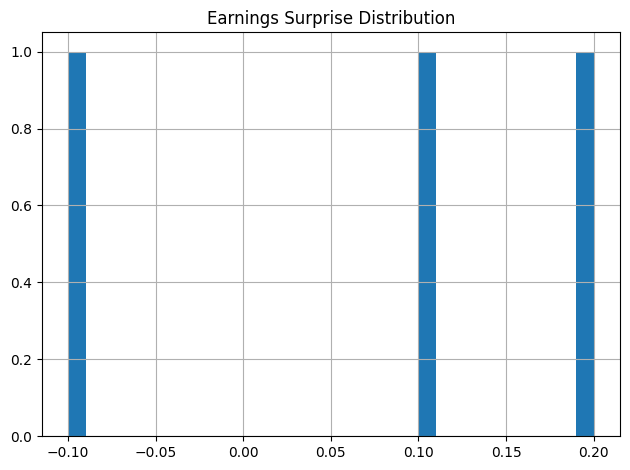
\includegraphics[keepaspectratio]{main_files/figure-pdf/cell-7-output-1.png}}

\begin{Highlighting}
\textcolor{black}{: }
\textcolor{black}{}\textcolor{QuartoInternalColor1}{notebook controller is DISPOSED. }
\textcolor{QuartoInternalColor1}{}\textcolor{QuartoInternalColor1}{View Jupyter <a href='command:jupyter.viewOutput'>log</a> for further details.}
\end{Highlighting}

\begin{Highlighting}
\textcolor{black}{: }
\textcolor{black}{}\textcolor{QuartoInternalColor1}{notebook controller is DISPOSED. }
\textcolor{QuartoInternalColor1}{}\textcolor{QuartoInternalColor1}{View Jupyter <a href='command:jupyter.viewOutput'>log</a> for further details.}
\end{Highlighting}

Models

\begin{itemize}
\tightlist
\item
  Baselines: Start with simple baselines (mean/last value,
  logistic/linear).
\item
  Candidates: Consider tree-based (RF/XGBoost), linear, neural, or
  specialized models.
\item
  Hyperparameters: Document search space and defaults.
\end{itemize}

\begin{center}\rule{0.5\linewidth}{0.5pt}\end{center}

\begin{itemize}
\tightlist
\item
  Experiment Plan: A compact matrix listing planned model families, key
  features, and parameters to try.
\end{itemize}

Training

\begin{itemize}
\tightlist
\item
  Strategy: Train/validation/test split strategy, cross-validation, and
  seeds.
\item
  Reproducibility: Deterministic seeds, config files, and artifact
  logging.
\item
  Compute: Hardware, runtime, and cost notes.
\end{itemize}

\begin{center}\rule{0.5\linewidth}{0.5pt}\end{center}

\begin{itemize}
\tightlist
\item
  Split Strategy \& Leakage: Explicitly state split logic (time-aware vs
  random), test size, and leakage mitigations.
\item
  Reproducibility Checklist: Config use, seeds, artifact locations,
  environment capture (Python + key pkg versions).
\end{itemize}

\begin{Shaded}
\begin{Highlighting}[]
\CommentTok{\# Train model using generated features}
\ImportTok{import}\NormalTok{ sys}
\ImportTok{from}\NormalTok{ pathlib }\ImportTok{import}\NormalTok{ Path}
\NormalTok{sys.path.append(}\BuiltInTok{str}\NormalTok{(Path.cwd() }\OperatorTok{/} \StringTok{\textquotesingle{}src\textquotesingle{}}\NormalTok{))}
\ImportTok{from}\NormalTok{ yourproj.train }\ImportTok{import}\NormalTok{ main }\ImportTok{as}\NormalTok{ train\_main}
\NormalTok{CONFIG }\OperatorTok{=} \StringTok{\textquotesingle{}configs/exp\_baseline.yaml\textquotesingle{}}
\NormalTok{train\_main(CONFIG)}
\end{Highlighting}
\end{Shaded}

\begin{Shaded}
\begin{Highlighting}[]
\CommentTok{\# Evaluate model and save simple plots}
\ImportTok{import}\NormalTok{ sys}
\ImportTok{from}\NormalTok{ pathlib }\ImportTok{import}\NormalTok{ Path}
\NormalTok{sys.path.append(}\BuiltInTok{str}\NormalTok{(Path.cwd() }\OperatorTok{/} \StringTok{\textquotesingle{}src\textquotesingle{}}\NormalTok{))}
\ImportTok{from}\NormalTok{ yourproj.}\BuiltInTok{eval} \ImportTok{import}\NormalTok{ main }\ImportTok{as}\NormalTok{ eval\_main}
\NormalTok{CONFIG }\OperatorTok{=} \StringTok{\textquotesingle{}configs/exp\_baseline.yaml\textquotesingle{}}
\NormalTok{eval\_main(CONFIG)}
\end{Highlighting}
\end{Shaded}

\begin{verbatim}
Metrics: {'accuracy': 1.0, 'auc': None, 'features': ['surprise'], 'n_test': 1}
Saved artifacts/figures/metrics.pdf
\end{verbatim}

\pandocbounded{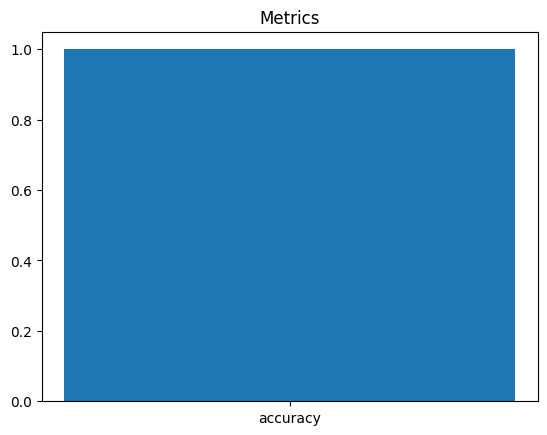
\includegraphics[keepaspectratio]{main_files/figure-pdf/cell-9-output-2.png}}

\begin{Highlighting}
\textcolor{black}{: }
\textcolor{black}{}\textcolor{QuartoInternalColor1}{notebook controller is DISPOSED. }
\textcolor{QuartoInternalColor1}{}\textcolor{QuartoInternalColor1}{View Jupyter <a href='command:jupyter.viewOutput'>log</a> for further details.}
\end{Highlighting}

\begin{Highlighting}
\textcolor{black}{: }
\textcolor{black}{}\textcolor{QuartoInternalColor1}{notebook controller is DISPOSED. }
\textcolor{QuartoInternalColor1}{}\textcolor{QuartoInternalColor1}{View Jupyter <a href='command:jupyter.viewOutput'>log</a> for further details.}
\end{Highlighting}

\begin{Highlighting}
\textcolor{black}{: }
\textcolor{black}{}\textcolor{QuartoInternalColor1}{notebook controller is DISPOSED. }
\textcolor{QuartoInternalColor1}{}\textcolor{QuartoInternalColor1}{View Jupyter <a href='command:jupyter.viewOutput'>log</a> for further details.}
\end{Highlighting}

Evaluation

\begin{itemize}
\tightlist
\item
  Metrics: Primary and secondary metrics; calibration and confidence
  intervals if applicable.
\item
  Error Analysis: Segment performance by cohort/time; investigate
  failure modes.
\item
  Reporting: Figures/tables for stakeholders and decision makers.
\end{itemize}

\begin{center}\rule{0.5\linewidth}{0.5pt}\end{center}

\begin{itemize}
\tightlist
\item
  Error Analysis Plan: Cohorts, time slices, and failure-mode checks
  (class imbalance, drift).
\item
  Decisions Log: A running list of major decisions with brief rationale
  (e.g., ``Chose chrono split due to event causality'').
\end{itemize}

Conclusion and Next Steps

Resources

\begin{itemize}
\item
  \textbf{TF--IDF Vectorizer API}\\
  Official docs for TfidfVectorizer (parameters like ngram\_range,
  min\_df, max\_features, etc.)\\
  https://scikit-learn.org/stable/modules/generated/sklearn.feature\_extraction.text.TfidfVectorizer.html
\item
  \textbf{Text Analytics Tutorial}\\
  End-to-end guide: load raw text, vectorize with TF--IDF, train a
  linear classifier\\
  https://scikit-learn.org/1.4/tutorial/text\_analytics/working\_with\_text\_data.html
\item
  \textbf{TF--IDF Math \& Intuition}\\
  Blog post with mathematical derivation, code examples, and visual
  intuition for term- and document-frequency weighting\\
  https://medium.com/@rohit\_batra/multi-class-text-classification-with-scikit-learn-using-tf-idf-model-161d395ce374
\item
  \textbf{Logistic Regression API}\\
  Full parameter reference (\texttt{solver}, \texttt{C},
  \texttt{penalty}, \texttt{class\_weight}, etc.) including valid ranges
  and examples\\
  https://scikit-learn.org/stable/modules/generated/sklearn.linear\_model.LogisticRegression.html
\end{itemize}




\end{document}
